In this section our infrastructure is presented. The theory behind it is based on the horseshoe modernization model, which is depicts in Figure~\ref{fig:horseshoe}. As can be seen, this model consist of three steps, \textbf{Reverse Engineering}, (\textit{ii}) \textbf{Restructuring}, and \textbf{Forward Engineering}. The first step is represented by the left side of the horseshoe, it analyzes the legacy system in order to identify the components of the system and their interrelationships. Usually the reverse engineering step builds one or more representations of the legacy system at a higher level of abstraction (PSM). The second one is represented by the curve of the horseshoe since this steps takes the previous system's representation (PSM) and transforms it into another one (\textbf{P}lataform \textbf{I}ndependent \textbf{M}odel - PIM) at the same abstraction level. Finally, the last step is represented by the right side of the horseshoe because it generates physical implementations (source-code) of the target system at a low abstraction level from the previously restructured representation of the system.

\begin{figure}[!h]
\centering
  % Requires \usepackage{graphicx}%left,bottom, right and top
 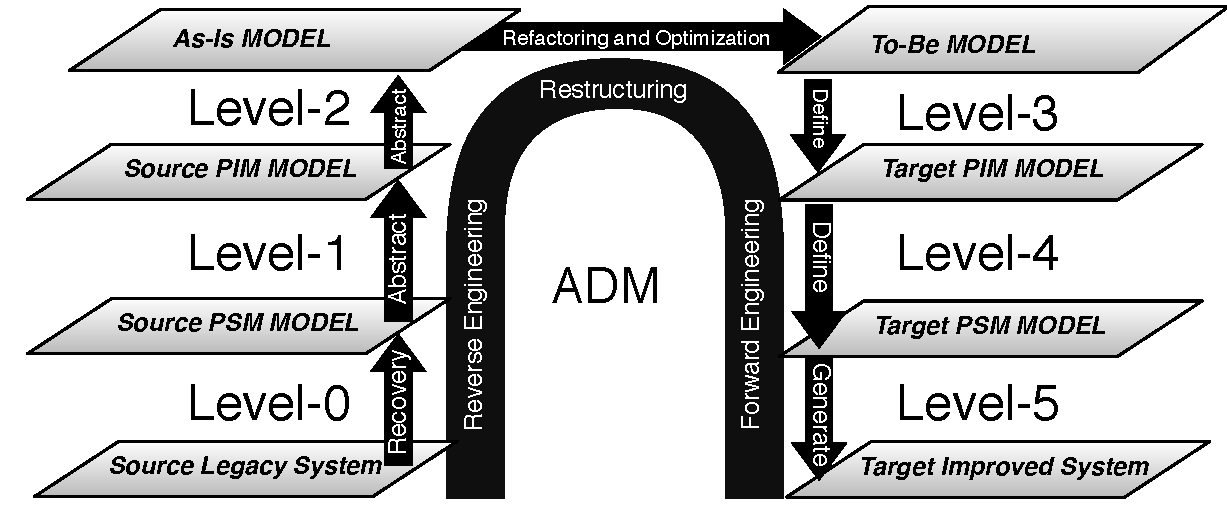
\includegraphics[%scale=0.063, clip=true, trim=32.23cm 18cm 5.45cm 13.853cm
 width=1\textwidth
 ]{Figuras/horseShoeBOM}
\caption{Horseshoe modernization model.}
\label{fig:horseshoe}
\end{figure}

It worth noticing that KDM is the most essential part of our infrastructure. KDM supplies the representation and management of knowledge extracted by means of reverse engineering from all the different software artifacts of the legacy system. Therefore, the legacy knowledge obtained is then modernized into a target improved system by using the concept of MDD. As the infrastructure herein follows the three steps depicts in Figure~\ref{fig:horseshoe} then it has to go through five abstraction levels with four transformations among them. In Figure~\ref{fig:infra} is depicted the infrastructure and also illustrates all abstract levels and the transformations (see the letters `A'- `F'). The Section~\ref{subsection:abstract_level} describes the abstract levels and the Section~\ref{subsection:transformation} explains the transformations.

\subsection{Abstract Levels}\label{subsection:abstract_level}
The \textbf{Level-0} represents all artifacts of the legacy systems in the real world, such as source code and database. The infrastructure uses this artifacts as input to start the ADM process.

The \textbf{Level-1} consist of two PSM model. The former model is a source code model, which represents all abstraction of the legacy system's source code, Figure~\ref{fig:infra}(B) illustrates it. More specifically, this model represents an \textbf{A}bstract \textbf{S}yntax \textbf{T}ree (AST), which is a tree representation of the abstract syntactic structure of Java source code. The latter is a database model that illustrates informations related to database used in the legacy system, see Figure~\ref{fig:infra}(A). Similarly, this model is also represented by an AST, the only difference is that it represents syntactic structure of database instead of Java source code. This database model is based on the SQL-92 Data Manipulation Language which can represent the SQL operations such as \textit{Select}, \textit{Delete}, \textit{Update} and \textit{Insert}. In order to transform the legacy system in these models it is necessary carry out a syntactical analyzer. As for the first model we used a parser that provides a complete self-describing representation of Java source code, i.e., this representation reflects the structure of the software artifact directly in the nesting of elements. Regarding the second model we devised a SQL parser. It consists of a extension of the previously parser but it intends to identify SQL embedded in the legacy system's source code. This parser focus on identifying SQL operations such as \textit{Select}, \textit{Delete}, \textit{Update} and \textit{Insert}; the tables, the columns, primary keys, etc, that appear in these SQL operations are then represented into a AST. Both models, the souce code model and the data base model  are represented in the XMI (\textbf{XM}L Metadata \textbf{I}nterchange)-based syntax as can be seen in Figure~\ref{fig:infra} (B) and Figure~\ref{fig:infra} (A), respectively.   


%Both models are deemed as PSM once they owns the software artifact according to their specific technology platforms. 

The \textbf{Level-2} consist of a single PIM which represents the integrated view of the set of PSM models in \textbf{Level-1}. It is based on the KDM specification once it makes possible to model all the artifacts of the legacy systems in an integrated and technological-independent way. A set of refactoring and optimizations is carried out by using this model. 


This model is based on the KDM specification. 


\subsection{Transformation}\label{subsection:transformation}






\begin{figure}[!h]
\centering
  % Requires \usepackage{graphicx}%left,bottom, right and top
 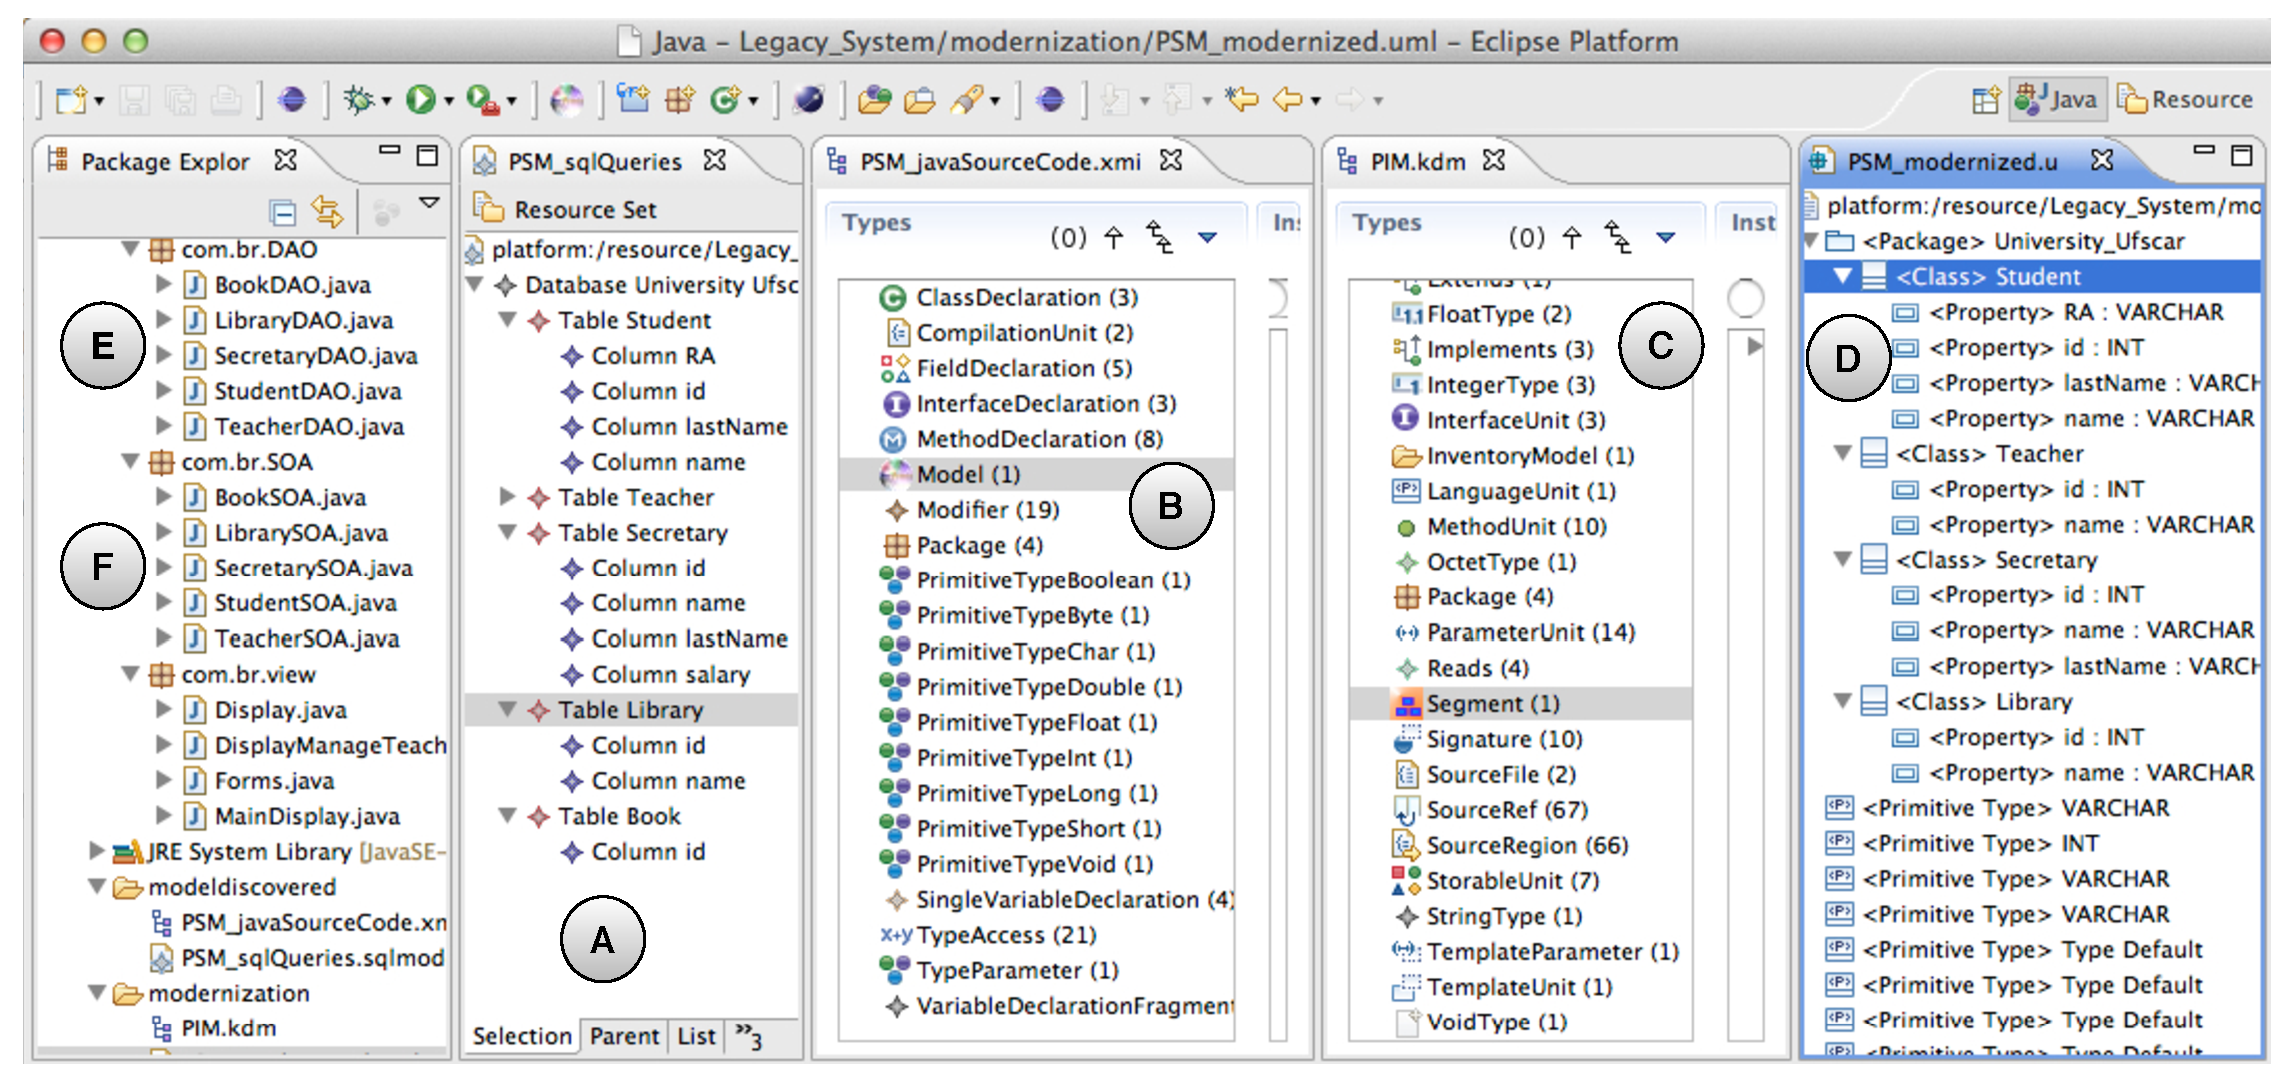
\includegraphics[%scale=0.063, clip=true, trim=32.23cm 18cm 5.45cm 13.853cm
 width=1\textwidth
 ]{Figuras/Tool}
\caption{Screenshot of the Infrastructure}
\label{fig:infra}
\end{figure}